% Created by tikzDevice version 0.12.6 on 2025-04-23 11:51:08
% !TEX encoding = UTF-8 Unicode
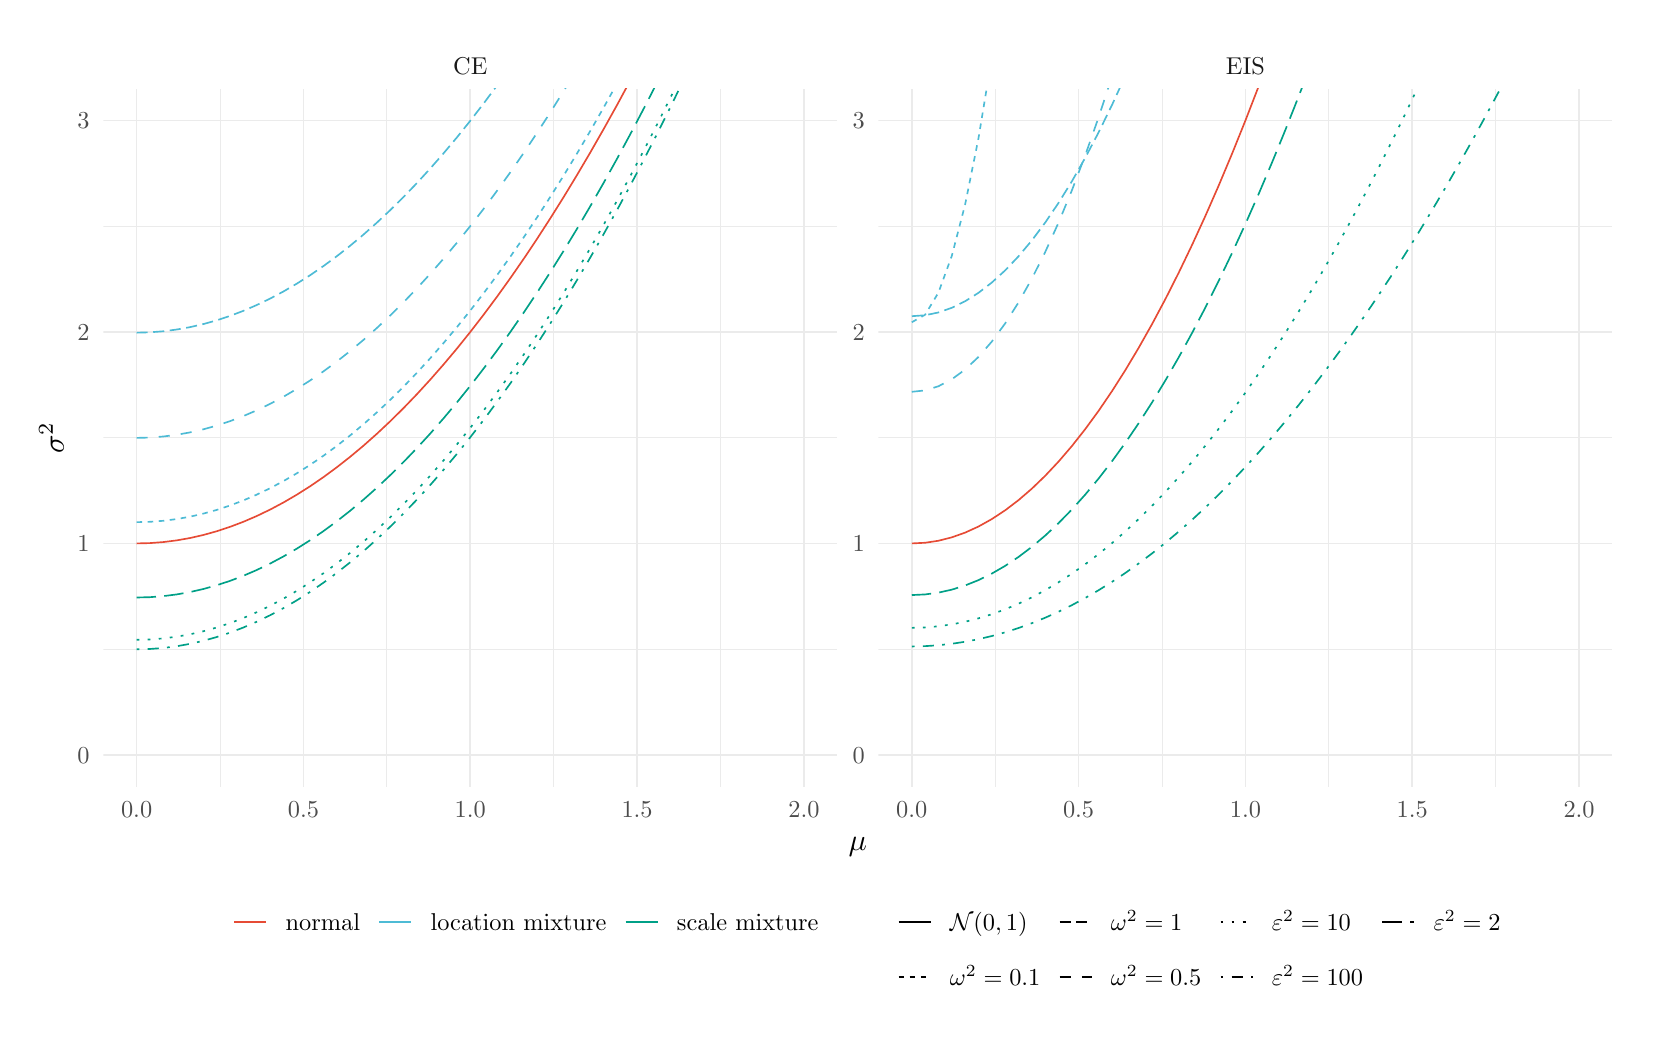
\begin{tikzpicture}[x=1pt,y=1pt]
\definecolor{fillColor}{RGB}{255,255,255}
\path[use as bounding box,fill=fillColor,fill opacity=0.00] (0,0) rectangle (578.16,361.35);
\begin{scope}
\path[clip] ( 27.31, 87.09) rectangle (292.56,339.28);
\definecolor{drawColor}{gray}{0.92}

\path[draw=drawColor,line width= 0.3pt,line join=round] ( 27.31,136.77) --
	(292.56,136.77);

\path[draw=drawColor,line width= 0.3pt,line join=round] ( 27.31,213.19) --
	(292.56,213.19);

\path[draw=drawColor,line width= 0.3pt,line join=round] ( 27.31,289.61) --
	(292.56,289.61);

\path[draw=drawColor,line width= 0.3pt,line join=round] ( 69.51, 87.09) --
	( 69.51,339.28);

\path[draw=drawColor,line width= 0.3pt,line join=round] (129.80, 87.09) --
	(129.80,339.28);

\path[draw=drawColor,line width= 0.3pt,line join=round] (190.08, 87.09) --
	(190.08,339.28);

\path[draw=drawColor,line width= 0.3pt,line join=round] (250.36, 87.09) --
	(250.36,339.28);

\path[draw=drawColor,line width= 0.6pt,line join=round] ( 27.31, 98.56) --
	(292.56, 98.56);

\path[draw=drawColor,line width= 0.6pt,line join=round] ( 27.31,174.98) --
	(292.56,174.98);

\path[draw=drawColor,line width= 0.6pt,line join=round] ( 27.31,251.40) --
	(292.56,251.40);

\path[draw=drawColor,line width= 0.6pt,line join=round] ( 27.31,327.82) --
	(292.56,327.82);

\path[draw=drawColor,line width= 0.6pt,line join=round] ( 39.37, 87.09) --
	( 39.37,339.28);

\path[draw=drawColor,line width= 0.6pt,line join=round] ( 99.65, 87.09) --
	( 99.65,339.28);

\path[draw=drawColor,line width= 0.6pt,line join=round] (159.94, 87.09) --
	(159.94,339.28);

\path[draw=drawColor,line width= 0.6pt,line join=round] (220.22, 87.09) --
	(220.22,339.28);

\path[draw=drawColor,line width= 0.6pt,line join=round] (280.51, 87.09) --
	(280.51,339.28);
\definecolor{drawColor}{RGB}{230,75,53}

\path[draw=drawColor,line width= 0.6pt,line join=round] ( 39.37,174.98) --
	( 44.19,175.10) --
	( 49.02,175.47) --
	( 53.84,176.08) --
	( 58.66,176.93) --
	( 63.48,178.03) --
	( 68.31,179.38) --
	( 73.13,180.97) --
	( 77.95,182.80) --
	( 82.77,184.88) --
	( 87.60,187.20) --
	( 92.42,189.77) --
	( 97.24,192.58) --
	(102.07,195.64) --
	(106.89,198.94) --
	(111.71,202.49) --
	(116.53,206.28) --
	(121.36,210.31) --
	(126.18,214.59) --
	(131.00,219.12) --
	(135.82,223.88) --
	(140.65,228.90) --
	(145.47,234.16) --
	(150.29,239.66) --
	(155.12,245.40) --
	(159.94,251.40) --
	(164.76,257.63) --
	(169.58,264.11) --
	(174.41,270.84) --
	(179.23,277.81) --
	(184.05,285.02) --
	(188.87,292.48) --
	(193.70,300.18) --
	(198.52,308.13) --
	(203.34,316.32) --
	(208.16,324.76) --
	(212.99,333.44) --
	(217.81,342.37) --
	(222.63,351.54) --
	(227.46,360.95) --
	(232.28,370.61) --
	(237.10,380.51) --
	(241.92,390.66) --
	(246.75,401.06) --
	(251.57,411.69) --
	(256.39,422.58) --
	(261.21,433.70) --
	(266.04,445.07) --
	(270.86,456.69) --
	(275.68,468.55) --
	(280.51,480.65);
\definecolor{drawColor}{RGB}{77,187,213}

\path[draw=drawColor,line width= 0.6pt,dash pattern=on 2pt off 2pt ,line join=round] ( 39.37,182.66) --
	( 44.19,182.79) --
	( 49.02,183.16) --
	( 53.84,183.78) --
	( 58.66,184.64) --
	( 63.48,185.75) --
	( 68.31,187.09) --
	( 73.13,188.69) --
	( 77.95,190.52) --
	( 82.77,192.61) --
	( 87.60,194.93) --
	( 92.42,197.50) --
	( 97.24,200.31) --
	(102.07,203.37) --
	(106.89,206.67) --
	(111.71,210.22) --
	(116.53,214.01) --
	(121.36,218.05) --
	(126.18,222.33) --
	(131.00,226.85) --
	(135.82,231.62) --
	(140.65,236.64) --
	(145.47,241.90) --
	(150.29,247.40) --
	(155.12,253.15) --
	(159.94,259.14) --
	(164.76,265.38) --
	(169.58,271.87) --
	(174.41,278.59) --
	(179.23,285.57) --
	(184.05,292.78) --
	(188.87,300.25) --
	(193.70,307.95) --
	(198.52,315.91) --
	(203.34,324.10) --
	(208.16,332.54) --
	(212.99,341.23) --
	(217.81,350.16) --
	(222.63,359.34) --
	(227.46,368.76) --
	(232.28,378.42) --
	(237.10,388.33) --
	(241.92,398.49) --
	(246.75,408.89) --
	(251.57,419.53) --
	(256.39,430.42) --
	(261.21,441.55) --
	(266.04,452.93) --
	(270.86,464.55) --
	(275.68,476.42) --
	(280.51,488.53);

\path[draw=drawColor,line width= 0.6pt,dash pattern=on 4pt off 2pt ,line join=round] ( 39.37,251.13) --
	( 44.19,251.27) --
	( 49.02,251.64) --
	( 53.84,252.27) --
	( 58.66,253.13) --
	( 63.48,254.24) --
	( 68.31,255.59) --
	( 73.13,257.19) --
	( 77.95,259.03) --
	( 82.77,261.12) --
	( 87.60,263.45) --
	( 92.42,266.02) --
	( 97.24,268.84) --
	(102.07,271.90) --
	(106.89,275.21) --
	(111.71,278.76) --
	(116.53,282.55) --
	(121.36,286.59) --
	(126.18,290.88) --
	(131.00,295.40) --
	(135.82,300.18) --
	(140.65,305.19) --
	(145.47,310.46) --
	(150.29,315.96) --
	(155.12,321.71) --
	(159.94,327.71) --
	(164.76,333.95) --
	(169.58,340.43) --
	(174.41,347.16) --
	(179.23,354.14) --
	(184.05,361.36) --
	(188.87,368.82) --
	(193.70,376.53) --
	(198.52,384.48) --
	(203.34,392.68) --
	(208.16,401.12) --
	(212.99,409.81) --
	(217.81,418.74) --
	(222.63,427.92) --
	(227.46,437.34) --
	(232.28,447.01) --
	(237.10,456.92) --
	(241.92,467.07) --
	(246.75,477.47) --
	(251.57,488.12) --
	(256.39,499.01) --
	(261.21,510.14) --
	(266.04,521.52) --
	(270.86,533.15) --
	(275.68,545.01) --
	(280.51,557.13);

\path[draw=drawColor,line width= 0.6pt,dash pattern=on 4pt off 4pt ,line join=round] ( 39.37,213.11) --
	( 44.19,213.24) --
	( 49.02,213.62) --
	( 53.84,214.24) --
	( 58.66,215.10) --
	( 63.48,216.21) --
	( 68.31,217.56) --
	( 73.13,219.16) --
	( 77.95,221.00) --
	( 82.77,223.08) --
	( 87.60,225.41) --
	( 92.42,227.98) --
	( 97.24,230.80) --
	(102.07,233.86) --
	(106.89,237.16) --
	(111.71,240.71) --
	(116.53,244.50) --
	(121.36,248.54) --
	(126.18,252.82) --
	(131.00,257.35) --
	(135.82,262.12) --
	(140.65,267.14) --
	(145.47,272.40) --
	(150.29,277.90) --
	(155.12,283.66) --
	(159.94,289.65) --
	(164.76,295.89) --
	(169.58,302.37) --
	(174.41,309.10) --
	(179.23,316.08) --
	(184.05,323.30) --
	(188.87,330.76) --
	(193.70,338.47) --
	(198.52,346.42) --
	(203.34,354.62) --
	(208.16,363.06) --
	(212.99,371.75) --
	(217.81,380.68) --
	(222.63,389.86) --
	(227.46,399.28) --
	(232.28,408.94) --
	(237.10,418.85) --
	(241.92,429.01) --
	(246.75,439.41) --
	(251.57,450.05) --
	(256.39,460.94) --
	(261.21,472.08) --
	(266.04,483.46) --
	(270.86,495.08) --
	(275.68,506.95) --
	(280.51,519.06);
\definecolor{drawColor}{RGB}{0,160,135}

\path[draw=drawColor,line width= 0.6pt,dash pattern=on 1pt off 3pt ,line join=round] ( 39.37,140.16) --
	( 44.19,140.29) --
	( 49.02,140.66) --
	( 53.84,141.28) --
	( 58.66,142.14) --
	( 63.48,143.24) --
	( 68.31,144.60) --
	( 73.13,146.19) --
	( 77.95,148.03) --
	( 82.77,150.12) --
	( 87.60,152.45) --
	( 92.42,155.02) --
	( 97.24,157.84) --
	(102.07,160.91) --
	(106.89,164.21) --
	(111.71,167.77) --
	(116.53,171.57) --
	(121.36,175.61) --
	(126.18,179.90) --
	(131.00,184.43) --
	(135.82,189.20) --
	(140.65,194.22) --
	(145.47,199.49) --
	(150.29,205.00) --
	(155.12,210.75) --
	(159.94,216.75) --
	(164.76,223.00) --
	(169.58,229.49) --
	(174.41,236.22) --
	(179.23,243.20) --
	(184.05,250.42) --
	(188.87,257.88) --
	(193.70,265.59) --
	(198.52,273.55) --
	(203.34,281.75) --
	(208.16,290.19) --
	(212.99,298.88) --
	(217.81,307.82) --
	(222.63,316.99) --
	(227.46,326.42) --
	(232.28,336.08) --
	(237.10,345.99) --
	(241.92,356.15) --
	(246.75,366.55) --
	(251.57,377.20) --
	(256.39,388.09) --
	(261.21,399.22) --
	(266.04,410.60) --
	(270.86,422.22) --
	(275.68,434.09) --
	(280.51,446.20);

\path[draw=drawColor,line width= 0.6pt,dash pattern=on 1pt off 3pt on 4pt off 3pt ,line join=round] ( 39.37,136.71) --
	( 44.19,136.84) --
	( 49.02,137.21) --
	( 53.84,137.83) --
	( 58.66,138.69) --
	( 63.48,139.80) --
	( 68.31,141.15) --
	( 73.13,142.75) --
	( 77.95,144.60) --
	( 82.77,146.68) --
	( 87.60,149.02) --
	( 92.42,151.59) --
	( 97.24,154.41) --
	(102.07,157.48) --
	(106.89,160.79) --
	(111.71,164.35) --
	(116.53,168.15) --
	(121.36,172.19) --
	(126.18,176.48) --
	(131.00,181.02) --
	(135.82,185.79) --
	(140.65,190.82) --
	(145.47,196.08) --
	(150.29,201.60) --
	(155.12,207.35) --
	(159.94,213.35) --
	(164.76,219.60) --
	(169.58,226.09) --
	(174.41,232.82) --
	(179.23,239.80) --
	(184.05,247.02) --
	(188.87,254.49) --
	(193.70,262.20) --
	(198.52,270.16) --
	(203.34,278.36) --
	(208.16,286.81) --
	(212.99,295.50) --
	(217.81,304.43) --
	(222.63,313.61) --
	(227.46,323.03) --
	(232.28,332.70) --
	(237.10,342.61) --
	(241.92,352.77) --
	(246.75,363.17) --
	(251.57,373.82) --
	(256.39,384.71) --
	(261.21,395.85) --
	(266.04,407.23) --
	(270.86,418.85) --
	(275.68,430.72) --
	(280.51,442.83);

\path[draw=drawColor,line width= 0.6pt,dash pattern=on 7pt off 3pt ,line join=round] ( 39.37,155.44) --
	( 44.19,155.56) --
	( 49.02,155.94) --
	( 53.84,156.55) --
	( 58.66,157.41) --
	( 63.48,158.51) --
	( 68.31,159.86) --
	( 73.13,161.45) --
	( 77.95,163.29) --
	( 82.77,165.37) --
	( 87.60,167.70) --
	( 92.42,170.27) --
	( 97.24,173.08) --
	(102.07,176.14) --
	(106.89,179.44) --
	(111.71,182.99) --
	(116.53,186.78) --
	(121.36,190.82) --
	(126.18,195.10) --
	(131.00,199.63) --
	(135.82,204.40) --
	(140.65,209.42) --
	(145.47,214.68) --
	(150.29,220.19) --
	(155.12,225.94) --
	(159.94,231.93) --
	(164.76,238.17) --
	(169.58,244.66) --
	(174.41,251.39) --
	(179.23,258.36) --
	(184.05,265.58) --
	(188.87,273.04) --
	(193.70,280.75) --
	(198.52,288.70) --
	(203.34,296.90) --
	(208.16,305.34) --
	(212.99,314.02) --
	(217.81,322.96) --
	(222.63,332.13) --
	(227.46,341.55) --
	(232.28,351.21) --
	(237.10,361.12) --
	(241.92,371.28) --
	(246.75,381.68) --
	(251.57,392.32) --
	(256.39,403.21) --
	(261.21,414.34) --
	(266.04,425.71) --
	(270.86,437.33) --
	(275.68,449.20) --
	(280.51,461.31);
\end{scope}
\begin{scope}
\path[clip] (307.41, 87.09) rectangle (572.66,339.28);
\definecolor{drawColor}{gray}{0.92}

\path[draw=drawColor,line width= 0.3pt,line join=round] (307.41,136.77) --
	(572.66,136.77);

\path[draw=drawColor,line width= 0.3pt,line join=round] (307.41,213.19) --
	(572.66,213.19);

\path[draw=drawColor,line width= 0.3pt,line join=round] (307.41,289.61) --
	(572.66,289.61);

\path[draw=drawColor,line width= 0.3pt,line join=round] (349.61, 87.09) --
	(349.61,339.28);

\path[draw=drawColor,line width= 0.3pt,line join=round] (409.89, 87.09) --
	(409.89,339.28);

\path[draw=drawColor,line width= 0.3pt,line join=round] (470.18, 87.09) --
	(470.18,339.28);

\path[draw=drawColor,line width= 0.3pt,line join=round] (530.46, 87.09) --
	(530.46,339.28);

\path[draw=drawColor,line width= 0.6pt,line join=round] (307.41, 98.56) --
	(572.66, 98.56);

\path[draw=drawColor,line width= 0.6pt,line join=round] (307.41,174.98) --
	(572.66,174.98);

\path[draw=drawColor,line width= 0.6pt,line join=round] (307.41,251.40) --
	(572.66,251.40);

\path[draw=drawColor,line width= 0.6pt,line join=round] (307.41,327.82) --
	(572.66,327.82);

\path[draw=drawColor,line width= 0.6pt,line join=round] (319.47, 87.09) --
	(319.47,339.28);

\path[draw=drawColor,line width= 0.6pt,line join=round] (379.75, 87.09) --
	(379.75,339.28);

\path[draw=drawColor,line width= 0.6pt,line join=round] (440.04, 87.09) --
	(440.04,339.28);

\path[draw=drawColor,line width= 0.6pt,line join=round] (500.32, 87.09) --
	(500.32,339.28);

\path[draw=drawColor,line width= 0.6pt,line join=round] (560.60, 87.09) --
	(560.60,339.28);
\definecolor{drawColor}{RGB}{230,75,53}

\path[draw=drawColor,line width= 0.6pt,line join=round] (319.47,174.98) --
	(324.29,175.22) --
	(329.11,175.95) --
	(333.94,177.18) --
	(338.76,178.89) --
	(343.58,181.09) --
	(348.40,183.78) --
	(353.23,186.96) --
	(358.05,190.63) --
	(362.87,194.78) --
	(367.69,199.43) --
	(372.52,204.57) --
	(377.34,210.19) --
	(382.16,216.30) --
	(386.99,222.91) --
	(391.81,230.00) --
	(396.63,237.58) --
	(401.45,245.65) --
	(406.28,254.21) --
	(411.10,263.26) --
	(415.92,272.79) --
	(420.74,282.82) --
	(425.57,293.34) --
	(430.39,304.34) --
	(435.21,315.83) --
	(440.04,327.82) --
	(444.86,340.29) --
	(449.68,353.25) --
	(454.50,366.70) --
	(459.33,380.64) --
	(464.15,395.06) --
	(468.97,409.98) --
	(473.79,425.39) --
	(478.62,441.28) --
	(483.44,457.67) --
	(488.26,474.54) --
	(493.09,491.90) --
	(497.91,509.76) --
	(502.73,528.10) --
	(507.55,546.93) --
	(512.38,566.24) --
	(517.20,586.05) --
	(522.02,606.35) --
	(526.84,627.14) --
	(531.67,648.41) --
	(536.49,670.18) --
	(541.31,692.43) --
	(546.14,715.17) --
	(550.96,738.40) --
	(555.78,762.12) --
	(560.60,786.33);
\definecolor{drawColor}{RGB}{77,187,213}

\path[draw=drawColor,line width= 0.6pt,dash pattern=on 2pt off 2pt ,line join=round] (319.47,254.90) --
	(324.29,257.62) --
	(329.11,265.62) --
	(333.94,278.91) --
	(338.76,297.51) --
	(343.58,321.43) --
	(348.40,350.70) --
	(353.23,385.32) --
	(358.05,425.30) --
	(362.87,470.66) --
	(367.69,521.41) --
	(372.52,577.55) --
	(377.34,639.10) --
	(382.16,706.06) --
	(386.99,778.45) --
	(391.81,856.27) --
	(396.63,939.53) --
	(401.45,1028.25) --
	(406.28,1122.43) --
	(411.10,1222.08) --
	(415.92,1327.22) --
	(420.74,1437.86) --
	(425.57,1554.00) --
	(430.39,1675.66) --
	(435.21,1802.84) --
	(440.04,1935.56) --
	(444.86,2073.83) --
	(449.68,2217.65) --
	(454.50,2367.05) --
	(459.33,2522.03) --
	(463.89,2673.99);

\path[draw=drawColor,line width= 0.6pt,dash pattern=on 4pt off 2pt ,line join=round] (319.47,257.09) --
	(324.29,257.43) --
	(329.11,258.44) --
	(333.94,260.13) --
	(338.76,262.50) --
	(343.58,265.54) --
	(348.40,269.26) --
	(353.23,273.66) --
	(358.05,278.74) --
	(362.87,284.49) --
	(367.69,290.93) --
	(372.52,298.06) --
	(377.34,305.86) --
	(382.16,314.36) --
	(386.99,323.53) --
	(391.81,333.39) --
	(396.63,343.94) --
	(401.45,355.18) --
	(406.28,367.10) --
	(411.10,379.71) --
	(415.92,393.00) --
	(420.74,406.99) --
	(425.57,421.66) --
	(430.39,437.02) --
	(435.21,453.06) --
	(440.04,469.80) --
	(444.86,487.22) --
	(449.68,505.33) --
	(454.50,524.12) --
	(459.33,543.61) --
	(464.15,563.78) --
	(468.97,584.64) --
	(473.79,606.19) --
	(478.62,628.42) --
	(483.44,651.34) --
	(488.26,674.95) --
	(493.09,699.25) --
	(497.91,724.23) --
	(502.73,749.90) --
	(507.55,776.26) --
	(512.38,803.31) --
	(517.20,831.04) --
	(522.02,859.46) --
	(526.84,888.57) --
	(531.67,918.36) --
	(536.49,948.84) --
	(541.31,980.01) --
	(546.14,1011.87) --
	(550.96,1044.41) --
	(555.78,1077.64) --
	(560.60,1111.56);

\path[draw=drawColor,line width= 0.6pt,dash pattern=on 4pt off 4pt ,line join=round] (319.47,229.77) --
	(324.29,230.27) --
	(329.11,231.78) --
	(333.94,234.30) --
	(338.76,237.83) --
	(343.58,242.38) --
	(348.40,247.93) --
	(353.23,254.50) --
	(358.05,262.08) --
	(362.87,270.68) --
	(367.69,280.30) --
	(372.52,290.94) --
	(377.34,302.60) --
	(382.16,315.28) --
	(386.99,328.98) --
	(391.81,343.71) --
	(396.63,359.46) --
	(401.45,376.23) --
	(406.28,394.02) --
	(411.10,412.84) --
	(415.92,432.68) --
	(420.74,453.54) --
	(425.57,475.43) --
	(430.39,498.34) --
	(435.21,522.27) --
	(440.04,547.23) --
	(444.86,573.21) --
	(449.68,600.21) --
	(454.50,628.24) --
	(459.33,657.29) --
	(464.15,687.37) --
	(468.97,718.46) --
	(473.79,750.59) --
	(478.62,783.73) --
	(483.44,817.90) --
	(488.26,853.09) --
	(493.09,889.31) --
	(497.91,926.55) --
	(502.73,964.82) --
	(507.55,1004.11) --
	(512.38,1044.42) --
	(517.20,1085.76) --
	(522.02,1128.12) --
	(526.84,1171.51) --
	(531.67,1215.92) --
	(536.49,1261.36) --
	(541.31,1307.83) --
	(546.14,1355.32) --
	(550.96,1403.83) --
	(555.78,1453.37) --
	(560.60,1503.94);
\definecolor{drawColor}{RGB}{0,160,135}

\path[draw=drawColor,line width= 0.6pt,dash pattern=on 1pt off 3pt ,line join=round] (319.47,144.47) --
	(324.29,144.62) --
	(329.11,145.04) --
	(333.94,145.73) --
	(338.76,146.68) --
	(343.58,147.91) --
	(348.40,149.40) --
	(353.23,151.17) --
	(358.05,153.21) --
	(362.87,155.51) --
	(367.69,158.09) --
	(372.52,160.95) --
	(377.34,164.07) --
	(382.16,167.47) --
	(386.99,171.14) --
	(391.81,175.08) --
	(396.63,179.30) --
	(401.45,183.79) --
	(406.28,188.55) --
	(411.10,193.58) --
	(415.92,198.89) --
	(420.74,204.47) --
	(425.57,210.32) --
	(430.39,216.44) --
	(435.21,222.83) --
	(440.04,229.49) --
	(444.86,236.43) --
	(449.68,243.63) --
	(454.50,251.10) --
	(459.33,258.84) --
	(464.15,266.85) --
	(468.97,275.13) --
	(473.79,283.68) --
	(478.62,292.50) --
	(483.44,301.58) --
	(488.26,310.93) --
	(493.09,320.55) --
	(497.91,330.43) --
	(502.73,340.58) --
	(507.55,351.00) --
	(512.38,361.68) --
	(517.20,372.63) --
	(522.02,383.84) --
	(526.84,395.32) --
	(531.67,407.06) --
	(536.49,419.07) --
	(541.31,431.34) --
	(546.14,443.88) --
	(550.96,456.68) --
	(555.78,469.74) --
	(560.60,483.07);

\path[draw=drawColor,line width= 0.6pt,dash pattern=on 1pt off 3pt on 4pt off 3pt ,line join=round] (319.47,137.75) --
	(324.29,137.87) --
	(329.11,138.19) --
	(333.94,138.72) --
	(338.76,139.45) --
	(343.58,140.38) --
	(348.40,141.52) --
	(353.23,142.86) --
	(358.05,144.42) --
	(362.87,146.17) --
	(367.69,148.14) --
	(372.52,150.31) --
	(377.34,152.69) --
	(382.16,155.28) --
	(386.99,158.08) --
	(391.81,161.09) --
	(396.63,164.30) --
	(401.45,167.73) --
	(406.28,171.36) --
	(411.10,175.20) --
	(415.92,179.25) --
	(420.74,183.51) --
	(425.57,187.98) --
	(430.39,192.65) --
	(435.21,197.53) --
	(440.04,202.62) --
	(444.86,207.92) --
	(449.68,213.42) --
	(454.50,219.13) --
	(459.33,225.05) --
	(464.15,231.17) --
	(468.97,237.50) --
	(473.79,244.03) --
	(478.62,250.77) --
	(483.44,257.72) --
	(488.26,264.87) --
	(493.09,272.22) --
	(497.91,279.78) --
	(502.73,287.54) --
	(507.55,295.51) --
	(512.38,303.68) --
	(517.20,312.05) --
	(522.02,320.63) --
	(526.84,329.41) --
	(531.67,338.40) --
	(536.49,347.58) --
	(541.31,356.97) --
	(546.14,366.56) --
	(550.96,376.36) --
	(555.78,386.35) --
	(560.60,396.55);

\path[draw=drawColor,line width= 0.6pt,dash pattern=on 7pt off 3pt ,line join=round] (319.47,156.32) --
	(324.29,156.55) --
	(329.11,157.20) --
	(333.94,158.28) --
	(338.76,159.79) --
	(343.58,161.72) --
	(348.40,164.09) --
	(353.23,166.88) --
	(358.05,170.10) --
	(362.87,173.75) --
	(367.69,177.82) --
	(372.52,182.33) --
	(377.34,187.27) --
	(382.16,192.64) --
	(386.99,198.44) --
	(391.81,204.66) --
	(396.63,211.32) --
	(401.45,218.40) --
	(406.28,225.91) --
	(411.10,233.85) --
	(415.92,242.22) --
	(420.74,251.01) --
	(425.57,260.23) --
	(430.39,269.88) --
	(435.21,279.95) --
	(440.04,290.45) --
	(444.86,301.37) --
	(449.68,312.72) --
	(454.50,324.48) --
	(459.33,336.68) --
	(464.15,349.29) --
	(468.97,362.33) --
	(473.79,375.79) --
	(478.62,389.67) --
	(483.44,403.97) --
	(488.26,418.70) --
	(493.09,433.84) --
	(497.91,449.41) --
	(502.73,465.39) --
	(507.55,481.79) --
	(512.38,498.62) --
	(517.20,515.86) --
	(522.02,533.52) --
	(526.84,551.60) --
	(531.67,570.09) --
	(536.49,589.00) --
	(541.31,608.33) --
	(546.14,628.08) --
	(550.96,648.24) --
	(555.78,668.82) --
	(560.60,689.81);
\end{scope}
\begin{scope}
\path[clip] ( 27.31,339.28) rectangle (292.56,355.85);
\definecolor{drawColor}{gray}{0.10}

\node[text=drawColor,anchor=base,inner sep=0pt, outer sep=0pt, scale=  0.88] at (159.94,344.53) {CE};
\end{scope}
\begin{scope}
\path[clip] (307.41,339.28) rectangle (572.66,355.85);
\definecolor{drawColor}{gray}{0.10}

\node[text=drawColor,anchor=base,inner sep=0pt, outer sep=0pt, scale=  0.88] at (440.04,344.53) {EIS};
\end{scope}
\begin{scope}
\path[clip] (  0.00,  0.00) rectangle (578.16,361.35);
\definecolor{drawColor}{gray}{0.30}

\node[text=drawColor,anchor=base,inner sep=0pt, outer sep=0pt, scale=  0.88] at ( 39.37, 76.08) {0.0};

\node[text=drawColor,anchor=base,inner sep=0pt, outer sep=0pt, scale=  0.88] at ( 99.65, 76.08) {0.5};

\node[text=drawColor,anchor=base,inner sep=0pt, outer sep=0pt, scale=  0.88] at (159.94, 76.08) {1.0};

\node[text=drawColor,anchor=base,inner sep=0pt, outer sep=0pt, scale=  0.88] at (220.22, 76.08) {1.5};

\node[text=drawColor,anchor=base,inner sep=0pt, outer sep=0pt, scale=  0.88] at (280.51, 76.08) {2.0};
\end{scope}
\begin{scope}
\path[clip] (  0.00,  0.00) rectangle (578.16,361.35);
\definecolor{drawColor}{gray}{0.30}

\node[text=drawColor,anchor=base,inner sep=0pt, outer sep=0pt, scale=  0.88] at (319.47, 76.08) {0.0};

\node[text=drawColor,anchor=base,inner sep=0pt, outer sep=0pt, scale=  0.88] at (379.75, 76.08) {0.5};

\node[text=drawColor,anchor=base,inner sep=0pt, outer sep=0pt, scale=  0.88] at (440.04, 76.08) {1.0};

\node[text=drawColor,anchor=base,inner sep=0pt, outer sep=0pt, scale=  0.88] at (500.32, 76.08) {1.5};

\node[text=drawColor,anchor=base,inner sep=0pt, outer sep=0pt, scale=  0.88] at (560.60, 76.08) {2.0};
\end{scope}
\begin{scope}
\path[clip] (  0.00,  0.00) rectangle (578.16,361.35);
\definecolor{drawColor}{gray}{0.30}

\node[text=drawColor,anchor=base east,inner sep=0pt, outer sep=0pt, scale=  0.88] at (302.46, 95.53) {0};

\node[text=drawColor,anchor=base east,inner sep=0pt, outer sep=0pt, scale=  0.88] at (302.46,171.95) {1};

\node[text=drawColor,anchor=base east,inner sep=0pt, outer sep=0pt, scale=  0.88] at (302.46,248.37) {2};

\node[text=drawColor,anchor=base east,inner sep=0pt, outer sep=0pt, scale=  0.88] at (302.46,324.79) {3};
\end{scope}
\begin{scope}
\path[clip] (  0.00,  0.00) rectangle (578.16,361.35);
\definecolor{drawColor}{gray}{0.30}

\node[text=drawColor,anchor=base east,inner sep=0pt, outer sep=0pt, scale=  0.88] at ( 22.36, 95.53) {0};

\node[text=drawColor,anchor=base east,inner sep=0pt, outer sep=0pt, scale=  0.88] at ( 22.36,171.95) {1};

\node[text=drawColor,anchor=base east,inner sep=0pt, outer sep=0pt, scale=  0.88] at ( 22.36,248.37) {2};

\node[text=drawColor,anchor=base east,inner sep=0pt, outer sep=0pt, scale=  0.88] at ( 22.36,324.79) {3};
\end{scope}
\begin{scope}
\path[clip] (  0.00,  0.00) rectangle (578.16,361.35);
\definecolor{drawColor}{RGB}{0,0,0}

\node[text=drawColor,anchor=base,inner sep=0pt, outer sep=0pt, scale=  1.10] at (299.99, 64.05) {$\mu$};
\end{scope}
\begin{scope}
\path[clip] (  0.00,  0.00) rectangle (578.16,361.35);
\definecolor{drawColor}{RGB}{0,0,0}

\node[text=drawColor,rotate= 90.00,anchor=base,inner sep=0pt, outer sep=0pt, scale=  1.10] at ( 13.08,213.19) {$\sigma^2$};
\end{scope}
\begin{scope}
\path[clip] (  0.00,  0.00) rectangle (578.16,361.35);
\definecolor{drawColor}{RGB}{230,75,53}

\path[draw=drawColor,line width= 0.6pt,line join=round] ( 74.73, 38.18) -- ( 86.29, 38.18);
\end{scope}
\begin{scope}
\path[clip] (  0.00,  0.00) rectangle (578.16,361.35);
\definecolor{drawColor}{RGB}{77,187,213}

\path[draw=drawColor,line width= 0.6pt,line join=round] (127.09, 38.18) -- (138.65, 38.18);
\end{scope}
\begin{scope}
\path[clip] (  0.00,  0.00) rectangle (578.16,361.35);
\definecolor{drawColor}{RGB}{0,160,135}

\path[draw=drawColor,line width= 0.6pt,line join=round] (216.11, 38.18) -- (227.67, 38.18);
\end{scope}
\begin{scope}
\path[clip] (  0.00,  0.00) rectangle (578.16,361.35);
\definecolor{drawColor}{RGB}{0,0,0}

\node[text=drawColor,anchor=base west,inner sep=0pt, outer sep=0pt, scale=  0.88] at ( 93.24, 35.15) {normal};
\end{scope}
\begin{scope}
\path[clip] (  0.00,  0.00) rectangle (578.16,361.35);
\definecolor{drawColor}{RGB}{0,0,0}

\node[text=drawColor,anchor=base west,inner sep=0pt, outer sep=0pt, scale=  0.88] at (145.60, 35.15) {location mixture};
\end{scope}
\begin{scope}
\path[clip] (  0.00,  0.00) rectangle (578.16,361.35);
\definecolor{drawColor}{RGB}{0,0,0}

\node[text=drawColor,anchor=base west,inner sep=0pt, outer sep=0pt, scale=  0.88] at (234.62, 35.15) {scale mixture};
\end{scope}
\begin{scope}
\path[clip] (  0.00,  0.00) rectangle (578.16,361.35);
\definecolor{drawColor}{RGB}{0,0,0}

\path[draw=drawColor,line width= 0.6pt,line join=round] (314.71, 38.18) -- (326.28, 38.18);
\end{scope}
\begin{scope}
\path[clip] (  0.00,  0.00) rectangle (578.16,361.35);
\definecolor{drawColor}{RGB}{0,0,0}

\path[draw=drawColor,line width= 0.6pt,dash pattern=on 2pt off 2pt ,line join=round] (314.71, 18.23) -- (326.28, 18.23);
\end{scope}
\begin{scope}
\path[clip] (  0.00,  0.00) rectangle (578.16,361.35);
\definecolor{drawColor}{RGB}{0,0,0}

\path[draw=drawColor,line width= 0.6pt,dash pattern=on 4pt off 2pt ,line join=round] (372.89, 38.18) -- (384.45, 38.18);
\end{scope}
\begin{scope}
\path[clip] (  0.00,  0.00) rectangle (578.16,361.35);
\definecolor{drawColor}{RGB}{0,0,0}

\path[draw=drawColor,line width= 0.6pt,dash pattern=on 4pt off 4pt ,line join=round] (372.89, 18.23) -- (384.45, 18.23);
\end{scope}
\begin{scope}
\path[clip] (  0.00,  0.00) rectangle (578.16,361.35);
\definecolor{drawColor}{RGB}{0,0,0}

\path[draw=drawColor,line width= 0.6pt,dash pattern=on 1pt off 3pt ,line join=round] (431.06, 38.18) -- (442.62, 38.18);
\end{scope}
\begin{scope}
\path[clip] (  0.00,  0.00) rectangle (578.16,361.35);
\definecolor{drawColor}{RGB}{0,0,0}

\path[draw=drawColor,line width= 0.6pt,dash pattern=on 1pt off 3pt on 4pt off 3pt ,line join=round] (431.06, 18.23) -- (442.62, 18.23);
\end{scope}
\begin{scope}
\path[clip] (  0.00,  0.00) rectangle (578.16,361.35);
\definecolor{drawColor}{RGB}{0,0,0}

\path[draw=drawColor,line width= 0.6pt,dash pattern=on 7pt off 3pt ,line join=round] (489.50, 38.18) -- (501.06, 38.18);
\end{scope}
\begin{scope}
\path[clip] (  0.00,  0.00) rectangle (578.16,361.35);
\definecolor{drawColor}{RGB}{0,0,0}

\node[text=drawColor,anchor=base west,inner sep=0pt, outer sep=0pt, scale=  0.88] at (333.22, 35.15) {$\mathcal N (0, 1)$};
\end{scope}
\begin{scope}
\path[clip] (  0.00,  0.00) rectangle (578.16,361.35);
\definecolor{drawColor}{RGB}{0,0,0}

\node[text=drawColor,anchor=base west,inner sep=0pt, outer sep=0pt, scale=  0.88] at (333.22, 15.20) {$\omega^2 = 0.1$};
\end{scope}
\begin{scope}
\path[clip] (  0.00,  0.00) rectangle (578.16,361.35);
\definecolor{drawColor}{RGB}{0,0,0}

\node[text=drawColor,anchor=base west,inner sep=0pt, outer sep=0pt, scale=  0.88] at (391.39, 35.15) {$\omega^2 = 1$};
\end{scope}
\begin{scope}
\path[clip] (  0.00,  0.00) rectangle (578.16,361.35);
\definecolor{drawColor}{RGB}{0,0,0}

\node[text=drawColor,anchor=base west,inner sep=0pt, outer sep=0pt, scale=  0.88] at (391.39, 15.20) {$\omega^2= 0.5$};
\end{scope}
\begin{scope}
\path[clip] (  0.00,  0.00) rectangle (578.16,361.35);
\definecolor{drawColor}{RGB}{0,0,0}

\node[text=drawColor,anchor=base west,inner sep=0pt, outer sep=0pt, scale=  0.88] at (449.57, 35.15) {$\varepsilon^2 = 10$};
\end{scope}
\begin{scope}
\path[clip] (  0.00,  0.00) rectangle (578.16,361.35);
\definecolor{drawColor}{RGB}{0,0,0}

\node[text=drawColor,anchor=base west,inner sep=0pt, outer sep=0pt, scale=  0.88] at (449.57, 15.20) {$\varepsilon^2 = 100$};
\end{scope}
\begin{scope}
\path[clip] (  0.00,  0.00) rectangle (578.16,361.35);
\definecolor{drawColor}{RGB}{0,0,0}

\node[text=drawColor,anchor=base west,inner sep=0pt, outer sep=0pt, scale=  0.88] at (508.01, 35.15) {$\varepsilon^2 = 2$};
\end{scope}
\end{tikzpicture}
